\documentclass[12pt]{article}

\usepackage{hyperref}
\usepackage{siunitx}
\usepackage{graphicx}

\usepackage[style=ieee, backend=bibtex]{biblatex}
\renewcommand{\bibfont}{\small}
\addbibresource{notes.bib}


\title{Gazebo Motor \& Propeller Model Notes}

\author{Matthew Vernacchia\\
Department of Aeronautics and Astronautics, MIT}

\date{\today}


\begin{document}
\maketitle

\section{Physical Model}
Let's begin with a simple physical model of the propeller. A short introduction to propeller theory is presented in \cite{Unified}, and one can read more details in McCormick's book \cite{McCormick1979}. This model addresses the thrust and torque of a propeller which is moving through the air parallel to its axis of rotation.

The model uses the following variables:

\begin{itemize}
    \item $\rho$, the air density (units: \si{\kilogram\per\meter\cubed})
    \item $T$, the thrust generated by the propeller (units: \si{\newton})
    \item $Q$, the torque generated by the propeller (units: \si{\newton\meter})
    \item $P$, the power required to drive the propeller (units: \si{\watt}).
    \item $n$, the rotation rate of the propeller (units: \si{rev \per\second}), and $\omega$, the angular speed of the propeller (units: \si{\radian\per\second}). $\omega = 2 \pi n$.
    \item $v_\parallel$ or $v_0$, the velocity at which the propeller is moving into the air along the rotation axis of the propeller (units: \si{\meter\per\second})
    \item $D$, the propeller diameter (units: \si{\meter}).
\end{itemize}

To simulate the forces and moments on a quadrotor, we need to predict how $T$ and $Q$ vary with $n$. This is acomplished using four dimensionless parameters:

\begin{itemize}
    \item $J = v_0 / D n$, the advance ratio.
    \item $C_T = T / \rho n^2 D^4$, the thrust coefficient (this is denoted as $k_T$ in \cite{Unified}).
    \item $C_Q = Q / \rho n^2 D^5$, the thrust coefficient (this is denoted as $k_Q$ in \cite{Unified}).
    \item $C_P = P / \rho n^3 D^5$, the thrust coefficient (this is denoted as $k_P$ in \cite{Unified}).
\end{itemize}

The thrust, torque, and power coefficients depend on the advance ratio $J$ and the design of the propeller\footnote{The thrust, torque and power coefficients also depend on the Reynolds and Mach number at the tip of the propeller, but for most quadrotors this is a small effect.}. To estimate the thrust and torque, we need to look up $C_T(J)$ and $C_Q(J)$ for our propeller, and then use:

\begin{equation}
    T = C_T(J) \rho n^2 D^4
\end{equation}
\begin{equation}
    Q = C_Q(J) \rho n^2 D^5
\end{equation}


The power and torque coefficients for all propellers are related by the equation $C_Q = C_P / 2 \pi$. Proof:
\[
P = Q \omega = Q (2 \pi n)
\]

\[
C_Q = \frac{Q}{\rho n^2 D^5} \left( \frac{n}{n} \right) = \frac{P}{2 \pi \rho n^3 D^5}
\]

\begin{equation}
C_Q =  \frac{C_P}{2 \pi}
\end{equation}

Thus, while most references will list only $C_T(J)$ and $C_P(J)$, we can easily find $C_Q$.

This model was developed for fixed-wing aircraft, and assumes that the air velocity is parallel to the rotation axis of the propeller. For quadrotors, the air velocity can also have a significant component perpendicular to rotation axis. This produces a force perpendicular to the thrust called the `H-force'. There are more complex models that attempt to predict the H-force. \cite{2016arXiv160100733B} provides a detailed derivation from blade element theory, and equations 1-2 of \cite{martin:hal-00422423} give a low-order model valid around hovering.


\section{Propellers Data}

Now we need to look up $C_T(J)$ and $C_P(J)$. UIUC provides a database of such data for small UAV/model aircraft propellers, available at \url{https://m-selig.ae.illinois.edu/props/propDB.html} \footnote{I've also included a zip file of the database in my repository (\url{https://github.com/mvernacc/gazebo_motor_model_docs}).}

Figure \ref{fig:prop_data_example} shows typical plots from this database. At static conditions, $C_T$ usually between $0.05$ and $0.2$, and then declines almost linearly with increasing $J$. Zero thrust usually occurs at $J = \SIrange{0.5}{1.0}{}$. $C_P$ is typically $0.03$ to $0.3$ at static conditions, and plateaus then declines with increasing $J$.

\begin{figure}
    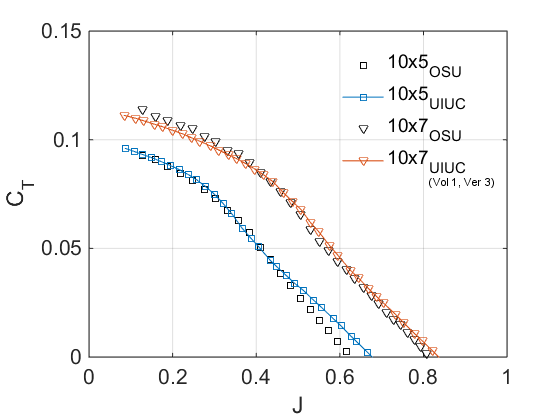
\includegraphics[width=0.5\textwidth]{UIUC-OSU-APC-E-comparison-June-2015-CT.png}
    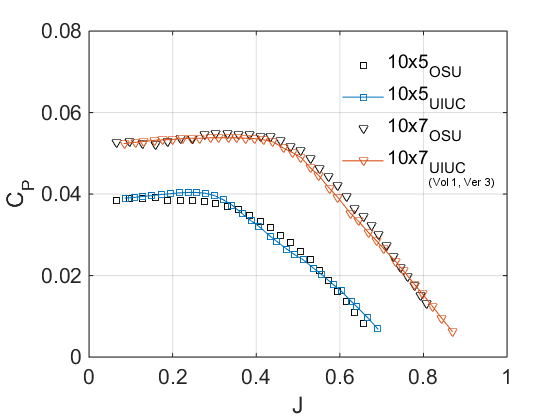
\includegraphics[width=0.5\textwidth]{UIUC-OSU-APC-E-comparison-June-2015-CP.png}
    \caption{\label{fig:prop_data_example} Example thrust and power coefficient data for two propellers (APC 10x5E and 10x7E). Reprinted from \cite{UIUCdatabase}.}
\end{figure}

In the US, propellers are designated by two numbers ``$D_{in} \times p_{in}$'', where $D_{in}$ is the diameter in inches and $p_{in}$ is the pitch in inches\footnote{The pitch angle $\beta$ is the angle bewteen the zero-lift line of the propeller blade section and the plane of rotation. The pitch $p$ is $p = \pi D \tan \beta$ for a constant-pitch propeller.} If you cannot find your vehicle's propeller in the database, use the data from a propeller design with similar ``$D_{in} \times p_{in}$''.

If no data is available, reasonable guesses for two-blade model aircraft propellers at $J=0$ (static) are $C_T = 0.1$ and $C_P = 0.05$ ($C_Q = 0.3$).

If you cannot find data for your propeller, you can also estimate the thrust and power coefficients using \emph{blade element theory}. This is rather involved. JavaProp (\url{https://www.mh-aerotools.de/airfoils/javaprop.htm}) is a free software package for perform these calculations.


\section{Current PX4 Gazebo SITL Model}

The source code for the PX4 Gazebo SITL motor/propeller model is available at \url{https://github.com/PX4/sitl_gazebo/blob/master/src/gazebo_motor_model.cpp}. This model uses notation that is different from the standard propeller model notation described above. Here I will attempt to provide a translation between the two models.

The thrust calculation is on \href{https://github.com/PX4/sitl_gazebo/blob/d08eb5b22d3edfb7a740c883b06f895a173b5519/src/gazebo_motor_model.cpp#L194}{line 194}:

\[
\mathtt{force = real\_motor\_velocity * real\_motor\_velocity * motor\_constant\_}
\]
Converting into the standard propeller model notation,
\[
T = \omega^2 (\mathtt{motor\_constant\_}) = (2 \pi n)^2 (\mathtt{motor\_constant\_}) = C_{T0} \rho n^2 D^4
\]
Thus,

\begin{equation}
\mathtt{motor\_constant\_} = \frac{C_{T0} \rho D^4}{(2 \pi)^2}
\end{equation}

where $C_{T0}$ is the static thrust coefficient at $J = 0$. This implies that \texttt{motor\_constant\_} has units of \si{\kilogram \meter}.  Note that \texttt{motor\_constant\_} is proportional to the fourth(!) power of propeller diameter, so using the same \texttt{motor\_constant\_} for propellers of different diameters is very inaccurate.

The Gazebo model then compensates for decreasing thrust at higher propeller/air velocities. It scales the force computed above by a value $\mathtt{scalar} \in [0, 1]$ (see \hyperref{https://github.com/PX4/sitl_gazebo/blob/d08eb5b22d3edfb7a740c883b06f895a173b5519/src/gazebo_motor_model.cpp#L204}{Lines 204-8}). The scaling parameter is set to

\[
\mathtt{scalar = 1 - vel / 25.0}
\]

and then clamped to the range $[0, 1]$. This vaguely captures the general trend of declining thrust at higher airspeeds. It is not an accurate implementation of the standard propeller model, but the standard propeller model will not make accurate thrust vs. airspeed predictions for quadrotors because there is a significant perpendicular velocity component.

The current Gazebo model also includes an `H-force' due to the perpendicular air velocity (see \href{https://github.com/PX4/sitl_gazebo/blob/d08eb5b22d3edfb7a740c883b06f895a173b5519/src/gazebo_motor_model.cpp#L221}{Line 221}), using a formula from equation 1 in \cite{martin:hal-00422423}:

\begin{equation}
H = - \omega \lambda_1 v_{\perp}
\end{equation}

The parameter $\lambda_1$ is (somewhat confusingly) called the \texttt{rotor\_drag\_coefficient\_} in the code.
The parameter $\lambda_1$ is \emph{not} dimensionless; it should have units of kilograms. No numerical values or physical relations for $\lambda_1$ are given in \cite{martin:hal-00422423}.
I do not know what value it should have or how it scales with rotor size \footnote{$\lambda_1 \sim \rho D^3$ would give the proper dimensionality.}. Perhaps \cite{2016arXiv160100733B} can give some insights?

The Gazebo model then computes the rotor torque magnitude to be \texttt{force * moment\_constant\_} (\href{https://github.com/PX4/sitl_gazebo/blob/d08eb5b22d3edfb7a740c883b06f895a173b5519/src/gazebo_motor_model.cpp#L233}{Line 233}). This implies that the \texttt{moment\_constant\_} has units of meters. Under the standard propeller theory, the \texttt{moment\_constant\_} should be:
\[
\mathtt{moment\_constant\_} = \frac{Q}{T} = \frac{C_{Q0} \rho n^2 D^5}{C_{T0} \rho n^2 D^4}
\]

\begin{equation}
\mathtt{moment\_constant\_} = \frac{C_{Q0}}{C_{T0}} D
\end{equation}

Finally, the Gazebo model adds a `rolling moment' (see \href{https://github.com/PX4/sitl_gazebo/blob/d08eb5b22d3edfb7a740c883b06f895a173b5519/src/gazebo_motor_model.cpp#L240}{Line 240}). The `rolling moment' is computed using the formula

\begin{equation}
M_{rolling} = - \omega \mu_1 v_\perp
\end{equation}

which is taken for equation 2 in \cite{martin:hal-00422423}.The parameter $\mu_1$ is not dimensionless; it has units of \si{\kilogram \meter}. Again, \cite{martin:hal-00422423} does not give numerical values or physical formulas for $\mu_1$, and I do not know how it scales with rotor size \footnote{$\mu_1 \sim \rho D^4$ would give the proper dimensionality.}
In the code, $\mu_1$ is referred to as \texttt{rolling\_moment\_coefficient\_}.


\section{Example for the Intel Aero Drone}
The Intel Aero Drone uses \SI{230}{\milli\meter} (9 inch) propellers from Yuneec. A spare parts seller for the Yuneec Typhoon H drone, which uses the same propellers, indicates that the propellers have pitch of 6 inches. There is a similar $9 \times 6$ propeller in the UIUC database (the APC Thin Electric $9 \times 6$), which has $C_{T0} = 0.11$ and $C_{P0} = 0.051$ ($C_{Q0} = 0.32$).

The $\mathtt{motor\_constant\_}$ is:

\begin{equation}
\mathtt{motor\_constant\_} = \frac{C_{T0} \rho D^4}{(2 \pi)^2} = \frac{0.11 (\SI{1.22}{\kilogram\per\meter\cubed}) (\SI{0.23}{\meter})^4}{(2 \pi)^2}
\end{equation}
\begin{equation}
\mathtt{motor\_constant\_} = \SI{9.5e-6}{\kilogram\meter}
\end{equation}

And the $\mathtt{moment\_constant\_}$ is:
\begin{equation}
\mathtt{moment\_constant\_} = \frac{C_{Q0}}{C_{T0}} D = \frac{0.32}{0.11} (\SI{0.23}{\meter})
\end{equation}
\begin{equation}
\mathtt{moment\_constant\_} = \SI{0.67}{\meter}
\end{equation}


\section{How to set the Model Parameters in the SDF File}
The Gazebo quadrotor model is defined in an SDF file for each aircraft. Within the SDF, there is a \texttt{plugin} block for each motor/propeller. These blocks start with the tag

\texttt{<plugin name='XXX' filename='libgazebo\_motor\_model.so'>}

where \texttt{XXX} is a unique name of the motor (see e.g. \href{https://github.com/PX4/sitl_gazebo/blob/d08eb5b22d3edfb7a740c883b06f895a173b5519/models/solo/solo.sdf#L358}{Line 358 of \texttt{solo.sdf}}). Within this block, their are tags for the \texttt{motorConstant} and \texttt{momentConstant} (the variables are named in camelCase in the SDF, but using underscores in the C++ code).

The model parameters are defined for each motor/propeller separately, so if you edit the file you will have to change the value in four places (for an aircraft with four propellers).

\printbibliography

\end{document}
